\Subsection{Prototipo Nido-Sustrato}
Para la construcción del prototipo del nido se tuvo en cuenta que el sustrato es de madera. Para las medidas se tuvieron en cuenta las disensiones promedio de un nido de carpintero \cite{ref:PaperValeriaOjeda}.

Por otro lado para alojar y proteger la electrónica se contempló el desarrollo de encapsulados. Primero se trabajó con la \rspi y sus complementos. Se adaptó un diseño existente agrandando su tamaño para que puedan introducirse las placas requeridas, se extendieron y fabricaron ranuras para el conexionado y se agregó un soporte que permita atornillar el conjunto. Para los sensores, se diseñó otro contenedor el cual contempla ranuras para que la cámara y los demás componentes estén en contacto con el exterior y ranuras para el conexionado con la \rpi.

Finalmente el diseño del prototipo de nido, se puede observar en los planos especificados en las Figuras (\ref{fig:base_nido_plano}), (\ref{fig:tapa_nido_plano}) y (\ref{fig:explotado_nido_plano}), mientras que los encapsulados se encuentran en las Figuras (\ref{fig:RpiCasingBottom}), (\ref{fig:RpiCasingTop}), (\ref{fig:BasePlano}) y (\ref{fig:TapaPlano}).

\Subsection{Prototipo Nido-Electrónica}

\Subsubsection{\rspi}
Para el prototipo se utiliza una \rspi 3B, sobre la cual se desarrollan los \textit{drivers} de comunicación con los diversos sensores. Además se confeccionó un \textit{shield} (encapsulado), el cuál realiza el acondicionamiento de las señales e interfaz para la placa de sensores.
\begin{figure}[H]
	\centering
	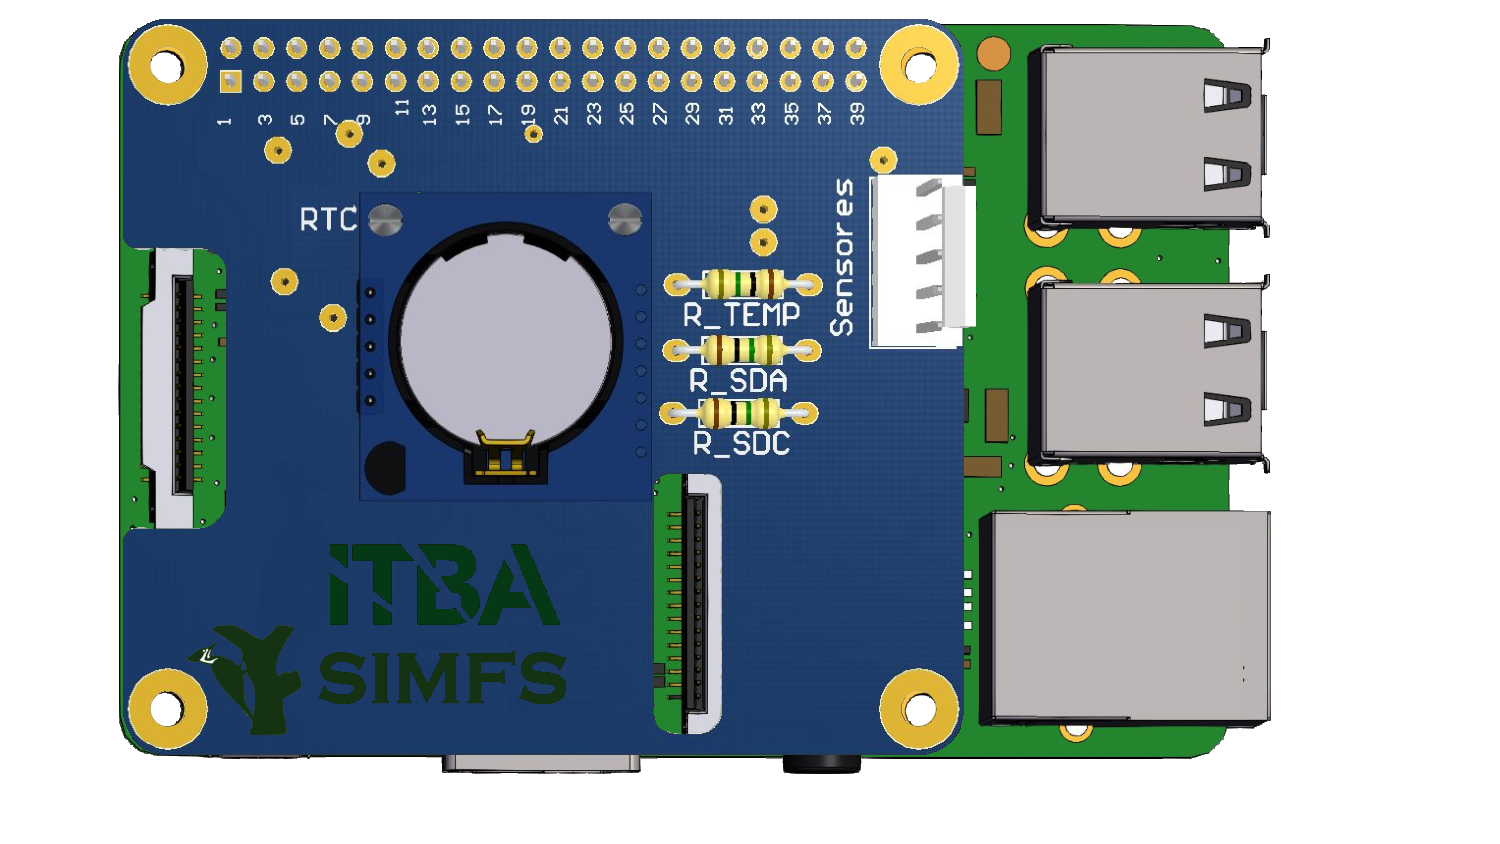
\includegraphics[width=0.9\linewidth,page=1]{ImagenesConstruccion del prototipo/shieldSensor}		
	\caption{Shield  y raspberry pi.}
	\label{fig:shield}
\end{figure}

\Subsubsection{Sensores}
En cuanto a los sensores se diseña una placa que se ubica en la bóveda del nido, la cual reúne todos los sensores necesarios, y ofrece una interfaz con la placa \textit{shield}.
\begin{figure}[H]
	\centering
	\includegraphics[width=0.9\linewidth,page=2]{ImagenesConstruccion del prototipo/shieldSensor}		
	\caption{Placa de sensores.}
	\label{fig:sens}
\end{figure}

\Subsection{Prototipo Nido-Potencia}
Para el prototipo del sistema de potencia del nido, se cuenta con la batería \TBC y la fuente simuladora de paneles solares \TBC.

\Subsection{Prototipo Nido-Comunicaciones }
Existen dos comunicaciones en el prototipo: la encargada de \nodered para comunicación con usuarios y la comunicación con la base principal de seguimiento para recolección de datos del ave.
